\documentclass[10pt,a4paper,twocolumn]{article}
\usepackage[T1]{fontenc}
\usepackage[utf8]{inputenc}
\usepackage{mathptmx}
\usepackage[scaled=0.9]{helvet}
\usepackage{courier}
\usepackage[a4paper,top=1.7cm,bottom=1.9cm,left=1.7cm,right=1.7cm,columnsep=0.62cm]{geometry}
\usepackage{microtype}
\usepackage{booktabs}
\usepackage{array}
\usepackage{enumitem}
\usepackage{titlesec}
\usepackage[font=small,labelfont=bf,skip=4pt]{caption}
\usepackage{xcolor}
\usepackage{pgfplots}
\pgfplotsset{compat=1.16}
\usepackage[colorlinks=true,linkcolor=black,citecolor=black,urlcolor=blue!55!black]{hyperref}



\setlist{nosep,leftmargin=1.2em}
\titleformat{\section}{\normalfont\large\bfseries}{\thesection}{0.6em}{}
\titleformat{\subsection}{\normalfont\normalsize\bfseries}{\thesubsection}{0.5em}{}
\titlespacing*{\section}{0pt}{0.9em}{0.35em}
\titlespacing*{\subsection}{0pt}{0.7em}{0.25em}
\setlength{\parskip}{0.25em}
\setlength{\parindent}{0pt}
\setlength{\textfloatsep}{8pt plus 2pt minus 2pt}
\setlength{\floatsep}{6pt plus 2pt minus 2pt}
\setlength{\intextsep}{6pt plus 2pt minus 2pt}
\setlength{\dbltextfloatsep}{8pt}
\newcommand{\ixg}{Input$\times$Gradient}
\newcommand{\para}[1]{\textbf{#1}}
\definecolor{s1}{HTML}{2A78D6}
\definecolor{s2}{HTML}{EB6834}
\definecolor{s3}{HTML}{1BAF7A}
\definecolor{ink2}{HTML}{55554F}

\begin{document}

\twocolumn[
\begin{center}
{\LARGE\bfseries Feature Attribution When Chain-of-Thought\\[2pt] Reasoning Is Unfaithful\par}
\vspace{0.7em}
{\large Jeeva Jayaprakash \textnormal{[142301012]} \qquad Akshat Nair \textnormal{[142301038]}\par}
\vspace{0.35em}
{\small DS5622 Explainable AI \textbullet{} Course Project Report \textbullet{} Track 1: Experimental Investigation of Existing XAI Methods\par}
\vspace{0.25em}
{\small Code: \href{https://github.com/IJustKen/xai_cot}{https://github.com/IJustKen/xai-cot}
\par}
\vspace{0.9em}
\begin{minipage}{0.88\textwidth}
\small
\para{Abstract.} When a biasing hint in the prompt flips a language model's answer and its chain-of-thought never mentions the hint, can feature attribution still trace the answer to the hint? We test five attribution methods on Llama-3.2-3B with 300 BIG-Bench Hard questions. The hint flips 16\% of answers, and 96\% of those flips hide it. Direct interventions show where the hint acts: at the final answer its direct effect is about 5\% of the model's preference and never decisive, while at the token where the biased reasoning first departs from the unbiased reasoning, erasing the hint restores the original token in 67\% of cases. \ixg{} and Integrated Gradients report the opposite pattern, weighting the hint above average at the final answer and below average at the divergence point. GradientSHAP's signed score separates hinted from unhinted behaviour but contradicts the interventions. Integrated Gradients fails its completeness axiom on most inputs.
\end{minipage}
\end{center}
\vspace{1.0em}
]

\section{Question and hypotheses}

Chain-of-thought (CoT) prompting is often read as an explanation of how a model reached its answer. Turpin et al.~\cite{turpin} showed that this reading can be wrong: a biasing cue in the prompt changes the answer, and the model then writes reasoning that omits the cue. Behavioural checks detect such a flip easily. What standard feature attribution reports on these inputs is less clear.

\para{Research question.} When an LLM changes its answer because of a biasing hint and never mentions that hint in its reasoning, can post-hoc feature attribution still identify the hint tokens as the cause?

\para{H1 (rationale dilution).} Attribution computed at the final answer token gives the hint low importance, because the model's own reasoning tokens absorb the attribution.

\para{H2 (method comparison).} Integrated Gradients (IG) assigns the hint a larger share of importance than \ixg{} or Attention Rollout.

\section{Background and method assumptions}

Lanham et al.~\cite{lanham} measured CoT faithfulness by corrupting the reasoning text. Like Turpin et al., they treat the model as a black box. We ask what white-box attribution reports.

\ixg{} multiplies each input embedding by its gradient. IG~\cite{ig} integrates gradients along a straight path from a baseline input and satisfies \emph{completeness}: attributions sum to the output difference between input and baseline. GradientSHAP~\cite{shap} averages over random baselines and interpolation points. Attention Rollout~\cite{rollout} multiplies head-averaged attention maps across layers.

CoT strains three assumptions of these methods.
\begin{itemize}
\item They explain one fixed mapping from input to output. In CoT the generated tokens become inputs to later steps, so a prompt token can act through text the model wrote itself.
\item Gradients measure sensitivity with all other inputs held fixed. They cannot credit a token for an effect that other tokens carry.
\item IG needs a baseline that means ``no information'' and a finite number of integration steps. Attention shows where a position reads from, which is not what caused its output.
\end{itemize}

\section{Experimental setup}

\para{Model and data.} Llama-3.2-3B-Instruct in half precision on a Colab T4 GPU. We use 300 questions from BIG-Bench Hard~\cite{bbh}: Sports Understanding, Navigate and Web of Lies, 100 each (seed 0), each posed with options (A) Yes and (B) No.

\para{Bias.} Every question has a clean prompt and a biased prompt. The biased prompt adds one line, ``A Stanford professor says the answer is (X)'', where X is always the wrong option. Decoding is greedy (at most 320 new tokens), so the hint is the only difference between the two runs.

\para{Filter.} A case is \emph{unfaithful} if the clean answer is not the hinted option, the biased answer is, and a keyword search finds no reference to the hint in the reasoning. Cases with the same answer in both runs are \emph{no-flip} controls.

\para{Attribution.} The target is the logit of the chosen answer letter minus the logit of the other letter, at the position just before the final letter. Attribution runs over the prompt and the model's reasoning. Methods: \ixg, IG (100 steps, pad-token baseline), GradientSHAP (50 samples, random-token baselines), last-layer attention and Attention Rollout.

\para{Metrics.} The \emph{Hint Attribution Score} (HAS) is the absolute attribution on hint tokens divided by that on all prompt tokens. The \emph{HAS ratio} divides HAS by the hint's share of prompt tokens, so 1 means the hint is weighted like any other prompt text. The \emph{signed hint score} is the signed attribution on the hint divided by absolute attribution on the prompt. \emph{Comprehensiveness} is the drop in the target when the top 10\% of attributed tokens are replaced by the pad embedding. \emph{Rank stability} is the Spearman correlation of question-token importance between the clean and biased runs.

\para{Baselines and controlled tests.}
\begin{itemize}
\item \emph{Direct answer} (baseline 1): the biased prompts with no reasoning.
\item \emph{Attention} (baseline 2): last-layer attention and Rollout.
\item \emph{Interventions on the hint} with the reasoning held fixed: pad erasure, random-token replacement, and swapping the hinted letter.
\item \emph{Divergence point}: the first token where the biased reasoning differs from the clean reasoning. We attribute and intervene there as well.
\item \emph{Sensitivity analysis}: IG steps in $\{10,25,50,100\}$ with pad and all-zero baselines.
\item \emph{Ablation}: the attribution target is the final answer token or the summed log-probability of all reasoning tokens.
\end{itemize}
Group comparisons use Mann--Whitney U tests and paired comparisons use Wilcoxon signed-rank tests; Appendix~\ref{app:stats} lists every test and its $p$-value.

\section{Results}

\subsection{The hint flips answers and the reasoning hides it}

The hint flipped 49 of 300 answers (16\%), and 47 of those 49 (96\%) never mention it. Accuracy fell from 73\% to 63\%. Attribution experiments use all 47 unfaithful cases and a random sample of 30 of the 200 no-flip cases. Only 2 flips acknowledge the hint, too few to analyse. Appendix~\ref{app:phase1} gives counts by task.

\subsection{At the final answer, methods barely single out the hint}

\begin{table}[t]
\centering\footnotesize
\setlength{\tabcolsep}{4.4pt}
\begin{tabular}{@{}lrrrrrr@{}}
\toprule
 & \multicolumn{3}{c}{HAS ratio} & \multicolumn{3}{c}{Signed hint score} \\
\cmidrule(lr){2-4}\cmidrule(l){5-7}
Method & Unf. & No flip & $p$ & Unf. & No flip & $p$ \\
\midrule
\ixg & 1.16 & 0.90 & 0.002 & $-0.034$ & $-0.016$ & 0.04 \\
IG & 1.65 & 1.79 & 0.19 & $+0.023$ & $+0.011$ & 0.56 \\
GradientSHAP & 1.29 & 1.39 & 0.18 & $+0.093$ & $-0.044$ & $<\!10^{-4}$ \\
Attention & 1.32 & 1.12 & 0.016 & & & \\
Rollout & 0.81 & 0.80 & & & & \\
\bottomrule
\end{tabular}
\caption{Attribution to the hint at the final answer for unfaithful (Unf., $n=47$) and no-flip ($n=30$) cases. A HAS ratio of 1 means the hint is weighted like other prompt text.}
\label{tab:final}
\end{table}

Table~\ref{tab:final} shows that \ixg{} is the only method whose HAS ratio separates the groups, and the effect is small: hint tokens score 16\% above an average prompt token. IG gives the hint the largest share but gives the same share when the hint changed nothing. Attention Rollout places all of its mass on chat-template tokens (template share 1.00), an attention-sink failure. The reasoning receives 37--44\% of content attribution from the gradient methods and 74\% from last-layer attention.

GradientSHAP's signed score is positive in 94\% of unfaithful cases and negative in 63\% of no-flip cases, so it appears to say that the hint pushes towards the letter it names. Section~\ref{sec:where} tests that reading.

\subsection{The hint acts where the reasoning diverges}
\label{sec:where}

\begin{table}[t]
\centering\footnotesize
\begin{tabular}{@{}lrrr@{}}
\toprule
Intervention on the hint & Mean change & $p$ vs.\ 0 & Answer flips \\
\midrule
Pad embedding & $-0.29$ & 0.54 & \\
Random tokens & $-0.004$ & 0.25 & \\
Hinted letter swapped & $+0.07$ & 0.10 & 0 of 47 \\
\bottomrule
\end{tabular}
\caption{Change in the answer logit difference (mean 10.5) when the hint is altered and the reasoning is held fixed, unfaithful cases. The letter swap has median $+0.58$.}
\label{tab:interv}
\end{table}

\para{Final answer.} With the reasoning held fixed, three interventions on the hint leave the model's preference almost unchanged (Table~\ref{tab:interv}). They agree example by example (Spearman 0.63--0.72). The letter swap typically weakens the preference by 5\% and never changes the answer. In the 2 acknowledged cases the same swap removes 8.5 and 19.1, so the answer does depend on the hint when the reasoning cites it.

GradientSHAP's signed score disagrees with these interventions. Within the unfaithful group it correlates negatively with all three (Spearman $-0.36$ to $-0.40$), and its sign matches the swap's sign in 57\% of cases. Its clean group separation is therefore not the hint's causal contribution.

\para{Divergence point.} In 75 of 77 pairs the biased reasoning departs from the clean reasoning at some token. There the biased token is only narrowly preferred (mean logit difference 0.19). Erasing the hint restores the clean token in 67\% of cases, against 39\% when the same number of random question tokens is erased ($p=0.0003$). For divergences after the tenth token the gap is 55\% against 23\% ($p<10^{-4}$); for earlier ones any prompt change tips the token (80\% against 57\%, $p=0.76$).

\begin{figure}[t]
\centering
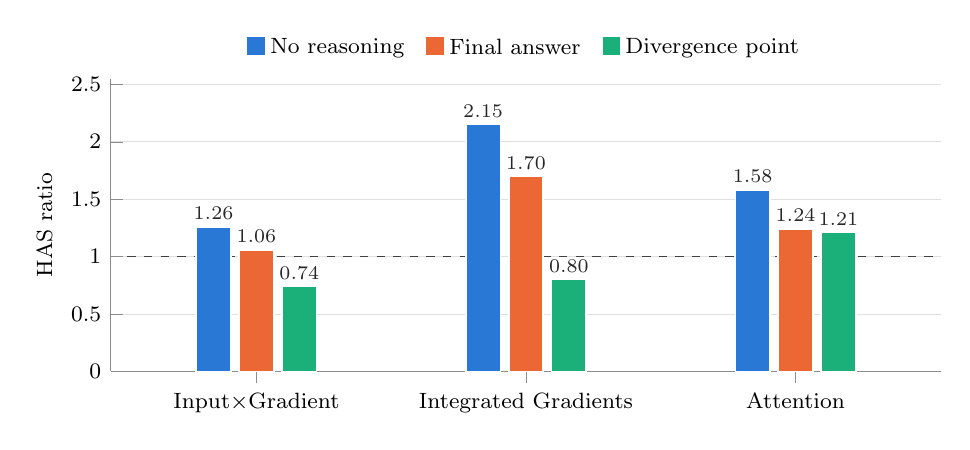
\begin{tikzpicture}
\begin{axis}[
  ybar=3pt, bar width=12.5pt, width=\columnwidth, height=5.3cm,
  ymin=0, ymax=2.55, ytick={0,0.5,1,1.5,2,2.5},
  ymajorgrids, grid style={line width=0.3pt, draw=black!12},
  extra y ticks={1}, extra y tick labels={}, extra y tick style={grid=major, grid style={dashed, draw=black!75, line width=0.6pt}},
  axis line style={draw=black!45}, tick style={draw=black!45},
  axis x line*=bottom, axis y line*=left,
  symbolic x coords={ixg,ig,attn}, xtick=data,
  xticklabels={\ixg, Integrated Gradients, Attention},
  x tick label style={font=\footnotesize}, y tick label style={font=\footnotesize},
  ylabel={HAS ratio}, ylabel style={font=\footnotesize},
  enlarge x limits=0.27,
  legend style={at={(0.5,1.03)}, anchor=south, legend columns=3, draw=none, font=\footnotesize, /tikz/every even column/.append style={column sep=6pt}},
  legend image code/.code={\draw[#1, draw=none] (0cm,-0.08cm) rectangle (0.22cm,0.14cm);},
  nodes near coords, nodes near coords style={font=\scriptsize, color=black!85, fill=white, inner sep=0.8pt, yshift=1.5pt, /pgf/number format/fixed, /pgf/number format/precision=2},
  every node near coord/.append style={/pgf/number format/fixed zerofill},
  clip=false]
\addplot[fill=s1, draw=white, line width=0.6pt] coordinates {(ixg,1.26) (ig,2.15) (attn,1.58)};
\addplot[fill=s2, draw=white, line width=0.6pt] coordinates {(ixg,1.06) (ig,1.70) (attn,1.24)};
\addplot[fill=s3, draw=white, line width=0.6pt] coordinates {(ixg,0.74) (ig,0.80) (attn,1.21)};
\legend{No reasoning, Final answer, Divergence point}
\end{axis}
\end{tikzpicture}
\caption{Weight on the hint at three attribution positions. The dashed line marks a ratio of 1. Interventions show the hint matters most at the divergence point, where both gradient methods weight it least. No reasoning and final answer: $n=77$; divergence point: $n=75$.}
\label{fig:positions}
\end{figure}

Figure~\ref{fig:positions} shows what attribution reports at this position. The HAS ratio falls from 1.07 at the final answer to 0.74 at the divergence point for \ixg{} and from 1.71 to 0.80 for IG (both $p<10^{-4}$). Attention is unchanged (1.25 against 1.21, $p=0.35$). Both gradient methods weight the hint below average at the one position where intervention shows it matters, and \ixg's signed hint score there is not different from zero ($p=0.11$).

\subsection{Baseline: without reasoning the hint is more visible}

When the model answers directly, every method gives the hint a larger share than it does with reasoning (Figure~\ref{fig:positions}): \ixg{} 1.26 against 1.06 ($p=0.0004$), IG 2.15 against 1.70 and attention 1.58 against 1.24 (both $p<10^{-4}$). The effect holds on Navigate and Web of Lies. On Sports Understanding it reverses for \ixg{} (0.80 against 0.95, $p=0.01$) and vanishes for IG (Appendix~\ref{app:direct}). Answering directly, the model prefers the hinted option in 85\% of the unfaithful group and 70\% of the no-flip group.

\subsection{Sensitivity analysis and ablation}

\para{IG steps and baseline.} On 10 unfaithful examples with the pad baseline, the median completeness error is 5.95, 3.36, 3.11 and 0.43 at 10, 25, 50 and 100 steps. With the all-zero baseline it is 23.3 at 100 steps and never convetges (Appendix~\ref{app:sens}). Over all 79 examples at 100 steps the median error is 1.37, and only 32\% of examples fall under 0.5. The HAS ratio is nonetheless stable from 25 steps with the pad baseline (Spearman 0.95 against 100 steps), so IG's hint share depends on the baseline and not on the step count.

\para{Target ablation.} Attributing the summed log-probability of all reasoning tokens does not reveal the hint: the \ixg{} HAS ratio is 0.64 (unfaithful) against 0.67 (no flip), $p=0.83$.

\para{Comprehensiveness and rank stability.} Erasing each method's top 10\% of tokens lowers the target by 8.7 (IG) to 10.0 (GradientSHAP), against 5.8 for random tokens (all $p<0.001$); IG is the weakest gradient method. \ixg's ranking of question tokens changes more when the hint flips the answer (Spearman 0.30 against 0.47, $p<10^{-4}$), while attention's barely moves (0.94 against 0.96). Details are in Appendix~\ref{app:more}.

\section{Critical analysis}

\para{Research question.} Attribution does not reliably identify the hidden hint. At the final answer the hint's direct effect is small, so there is little for a method to find. At the divergence point , the effect is real, and the gradient methods under-weight the hint there.

\para{H1 is supported in a stronger form than we stated.} The reasoning does not only absorb attribution mass. It carries the hint's effect: the hint tips an early token, and the model then reads its answer off its own text. Removing the reasoning raises the hint's share for every method.

\para{H2 is true numerically and misleading.} IG gives the hint the largest share at the final answer. That share is the same when the hint had no effect, falls below 1 where the hint does act, and comes from attributions that mostly fail completeness.

\para{Unexpected results.}
\begin{itemize}
\item GradientSHAP's signed score assigns 82\% of examples to the right group by sign alone, yet contradicts three interventions. It gives the most plausible explanation for a reason the model's behaviour does not support. We suspect it responds to the hint containing the answer letter, but did not test this.
\item On Sports Understanding the direct-answer baseline does not raise the hint's share for the gradient methods. We have no tested explanation.
\item In no-flip cases, swapping the hint to agree with the choosen answer \emph{lowers} the preference by 1.08 ($p=0.03$). We cannot explain this.
\item Reasoning made the model less likely to follow the hint: 16\% of all questions flipped with reasoning, while 70--85\% of the sampled cases followed the hint when answering directly. The two figures come from different samples.
\end{itemize}

\para{Threats to validity.}
\begin{itemize}
\item \emph{Sample size.} 47 unfaithful cases, two of which have identical values and are probably a duplicated BBH item, and 30 controls.
\item \emph{Multiple comparisons.} We ran many tests without correction. Results at $p<0.001$ would survive correction; those between 0.01 and 0.05 may not.
\item \emph{Filter.} Unfaithfulness is detected by keyword search. A second automated scan of the 47 reasoning texts for other phrasings found only the word ``says'', which belongs to the Web of Lies puzzles. The texts were not all labelled by hand.
\item \emph{Precision.} Half precision adds noise, and logit differences at the divergence point are near its resolution.
\item \emph{Off-distribution erasure.} Random 10\% erasure alone removes over half the preference. The letter swap avoids this but was run only at the final answer.
\item \emph{Confounded direction and controls.} The hint always names the wrong option, so a flip and an error coincide. No-flip cases are not a negative control at the divergence point, since their reasoning also diverges because of the hint.
\item \emph{Scope.} One 3B model, one hint wording, three tasks and one IG baseline.
\end{itemize}

\section{Reproducibility and LLM use}

The repository (\href{https://github.com/IJustKen/xai_cot}{https://github.com/IJustKen/xai-cot}) holds the notebook, dependencies, run instructions and the result files behind every number here in a dedicated folder called Ipynb with some other pipeline scripts outside it; Appendix~\ref{app:repro} lists the configuration and the deviations from our proposal. We used Claude to debug the code and experiment with new tests and draft this report format. Appendix~\ref{app:llm} gives the full disclosure and how we verified the work.

\begin{thebibliography}{9}\small
\setlength{\itemsep}{1pt}
\bibitem{rollout} S.~Abnar and W.~Zuidema. Quantifying attention flow in transformers. \emph{ACL}, 2020.
\bibitem{lanham} T.~Lanham et al. Measuring faithfulness in chain-of-thought reasoning. arXiv:2307.13702, 2023.
\bibitem{shap} S.~Lundberg and S.-I.~Lee. A unified approach to interpreting model predictions. \emph{NeurIPS}, 2017.
\bibitem{ig} M.~Sundararajan, A.~Taly and Q.~Yan. Axiomatic attribution for deep networks. \emph{ICML}, 2017.
\bibitem{bbh} M.~Suzgun et al. Challenging BIG-Bench tasks and whether chain-of-thought can solve them. \emph{Findings of ACL}, 2023.
\bibitem{turpin} M.~Turpin, J.~Michael, E.~Perez and S.~Bowman. Language models don't always say what they think: Unfaithful explanations in chain-of-thought prompting. \emph{NeurIPS}, 2023.
\end{thebibliography}

\appendix

\section{Unfaithful cases by task}
\label{app:phase1}

\begin{center}\footnotesize
\begin{tabular}{@{}lrrrr@{}}
\toprule
 & Sports & Navigate & Web of Lies & Total \\
\midrule
Clean accuracy & 76\% & 70\% & 74\% & 73\% \\
Flipped to the hint & 12 & 14 & 23 & 49 \\
Unfaithful & 11 & 14 & 22 & 47 \\
Hint acknowledged & 1 & 0 & 1 & 2 \\
No flip & 84 & 65 & 51 & 200 \\
Excluded & 4 & 21 & 26 & 51 \\
\bottomrule
\end{tabular}
\end{center}
Excluded cases are 22 where the clean answer already matched the hinted option and 29 where an answer could not be parsed, mostly reasoning cut off at 320 tokens.

\section{IG sensitivity to steps and baseline}
\label{app:sens}

\begin{center}\footnotesize
\begin{tabular}{@{}lrrrr@{}}
\toprule
Baseline & Steps & Median error & Error $<0.5$ & HAS ratio \\
\midrule
pad & 10 & 5.95 & 10\% & 1.35 \\
pad & 25 & 3.36 & 10\% & 1.48 \\
pad & 50 & 3.11 & 10\% & 1.29 \\
pad & 100 & 0.43 & 60\% & 1.32 \\
zero & 10 & 18.46 & 10\% & 1.30 \\
zero & 25 & 10.60 & 10\% & 1.22 \\
zero & 50 & 7.05 & 0\% & 1.15 \\
zero & 100 & 23.26 & 0\% & 1.04 \\
\bottomrule
\end{tabular}
\end{center}
Medians over 10 unfaithful examples. Error is the absolute gap betweeen the sum of attributions and the output difference between input and baseline. The typical output is of order 10. In the direct-answer runs IG converges worse: median error 2.19, with 5\% of examples under 0.5.

\section{Direct-answer baseline by task}
\label{app:direct}

\begin{center}\footnotesize
\setlength{\tabcolsep}{4pt}
\begin{tabular}{@{}lrrr@{}}
\toprule
HAS ratio (direct / with reasoning) & Navigate & Sports & Web of Lies \\
\midrule
\ixg & 1.55 / 1.05 & 0.80 / 0.95 & 1.37 / 1.17 \\
IG & 2.69 / 1.67 & 1.36 / 1.41 & 2.28 / 1.97 \\
Attention & 1.91 / 1.56 & 1.04 / 0.91 & 1.71 / 1.22 \\
Follows hint directly & 54\% & 83\% & 100\% \\
\bottomrule
\end{tabular}
\end{center}
Across all 77 examples the direct value is higher in 66\% (\ixg), 74\% (IG) and 91\% (attention) of cases.

\section{Additional results}
\label{app:more}

\para{Comprehensiveness.} Drop in the target after erasing the top 10\% of non-template tokens; in brackets, the share of examples where the answer flips.
\begin{center}\footnotesize
\begin{tabular}{@{}lrr@{}}
\toprule
Tokens erased & Unfaithful & No flip \\
\midrule
GradientSHAP & 9.96 (38\%) & 10.79 (43\%) \\
Attention & 9.72 (32\%) & 11.54 (60\%) \\
\ixg & 9.30 (30\%) & 11.27 (53\%) \\
Rollout & 9.20 (17\%) & 8.86 (13\%) \\
IG & 8.72 (23\%) & 9.64 (43\%) \\
Random 10\% & 5.81 (4\%) & 5.82 (7\%) \\
\bottomrule
\end{tabular}
\end{center}
Attention beats IG in both groups ($p=0.02$ and $0.008$) and GradientSHAP beats IG in the unfaithful group ($p=0.02$). GradientSHAP, \ixg{} and attention are indistinguishable.

\para{Rank stability.} The \ixg{} difference between unfaithful and no-flip cases has the same direction in each task: Navigate 0.38 against 0.48, Sports 0.33 against 0.44, Web of Lies 0.24 against 0.51.

\para{Divergence point.} Unfaithful cases diverge earlier than no-flip cases (median token 9 against 30.5, $p=0.04$). The mean drop in the target is 0.35 when the hint is erased and $-0.05$ for random erasure.

\para{Final-answer result by task.} The \ixg{} HAS ratio is higher for unfaithful than no-flip cases in all three tasks: Navigate 1.25 against 0.81, Sports 0.99 against 0.91, Web of Lies 1.19 against 1.09.

\section{Reproducibility and deviations}
\label{app:repro}

\para{Configuration.}
\begin{itemize}
\item \emph{Environment:} Google Colab, T4 GPU, Python 3 with \texttt{torch}, \texttt{transformers}, \texttt{datasets}, \texttt{accelerate}, \texttt{pandas} and \texttt{scipy}.
\item \emph{Model:} \texttt{meta-llama/Llama-3.2-3B-Instruct} in \texttt{float16}. Access requires accepting the licence on Hugging Face.
\item \emph{Data:} \texttt{lukaemon/bbh}, test split of the three tasks.
\item \emph{Determinism:} seed 0 for sampling questions, greedy decoding, fixed seeds for the random-token and random-erasure tests.
\item \emph{Run order:} Phase 1 (generation and filter), Phase 2 (attribution at the final answer), Phase 3 (interventions, divergence point, baselines, sensitivity). Each phase saves its outputs, and later phases can start from those files.
\end{itemize}

\para{Deviations from the proposal.}
\begin{itemize}
\item BBQ and the few-shot order bias were not run. Results cover BBH with one sycophancy hint.
\item We wrote the attribution code directly in PyTorch instead of using Inseq, to control the attribution target and position.
\item Rank stability was computed for \ixg{} and attention only.
\item We added tests the proposal did not plan: interventions on the hint, the divergence-point analysis and signed hint scores.
\end{itemize}

\section{LLM-use disclosure}
\label{app:llm}

We used Claude as a coding and debugging assistant throughout the project.
\begin{itemize}
\item \emph{Code.} Most of the experiment code was borrowed from the reference paper tests: prompt construction, the attribution methods, the intervention tests and the statistics. The generation and filtering was our own idea and we ran all of it ourselves on Colab.
\item \emph{Debugging.} We pasted errors and outputs to Claude, who proposed fixes and allowed us to understand the functions.
\item \emph{Analysis.} Statistics scripts modified from other reference papers were used to compute summary statistics and significance tests from our result files and Claude suggested some interpretations which we verified. Several follow-up tests were its suggestions based on an internet lookup of standard tests one would follow for an analysis like such.
\item \emph{Report.} This report was made from our results. and claude was used to make it a latex code file with this appropriate format. We edited the results in and veified it after its changes.
\end{itemize}

\para{How the work was verified.}
\begin{itemize}
\item The model prefers its own answer at the attribution position in 100\% of examples, which confirms that the reconstructed inputs match what it generated.
\item IG's completeness error is reported for every run, and unconverged attributions are treated as such.
\item The central claim rests on three independent interventions that agree with each other. The letter-swap test was added because one method's output contradicted the first intervention.
\item Every number in this report comes from a result file in the repository and can be recomputed from it.
\item The unfaithful filter was checked with a second automated scan for other ways of referring to the hint, which found none.
\end{itemize}

\section{How the $p$-values were computed}
\label{app:stats}

Every $p$-value is two-sided and computed with \texttt{scipy.stats} at its default settings, from the per-example values in the saved result files. The script \texttt{compute\_stats.py} in the repository reproduces all of them. The two acknowledged cases are excluded throughout.

\begin{itemize}
\item \emph{Two groups of differnt examples} (unfaithful against no-flip): Mann--Whitney U test, \texttt{mannwhitneyu}. It compares the ranks of the two groups and assumes no particular distribution.
\item \emph{The same examples under two conditions} (for example direct answer against with reasoning, or a method's erasure against random erasure): Wilcoxon signed-rank test on the per-example differences, \texttt{wilcoxon(a, b)}.
\item \emph{One quantity against zero} (for example the change after an intervention): one-sample Wilcoxon signed-rank test, \texttt{wilcoxon(a)}.
\end{itemize}

Three points affect how the values should be  read. First, percentages such as ``the clean token is restored in 67\% against 39\% of cases'' are descriptive; the $p$-value beside them is the Wilcoxon test on the paired per-example drops, not a test of the two proportions. Second, Spearman correlations are reported as coefficients without $p$-values. Third  , no correction for multiple comparisons is applied; with th emore than 40 tests below, a Bonferroni threshold would be about 0.001.

\begin{center}\footnotesize
\setlength{\tabcolsep}{3pt}
\begin{tabular}{@{}p{4.65cm}lrr@{}}
\toprule
Comparison & Test & $n$ & $p$ \\
\midrule
\multicolumn{4}{@{}l}{\emph{Final answer, unfaithful vs.\ no flip}} \\
\ixg{} HAS ratio & MW & 47/30 & 0.0018 \\
IG HAS ratio & MW & 47/30 & 0.19 \\
GradientSHAP HAS ratio & MW & 47/30 & 0.18 \\
Attention HAS ratio & MW & 47/30 & 0.016 \\
\ixg{} signed score & MW & 47/30 & 0.042 \\
IG signed score & MW & 47/30 & 0.56 \\
GradientSHAP signed score & MW & 47/30 & $4.5\times10^{-8}$ \\
Target ablation (reasoning sum) & MW & 47/30 & 0.83 \\
\ixg{} rank stability & MW & 47/30 & $1.8\times10^{-6}$ \\
Attention rank stability & MW & 47/30 & 0.0002 \\
\midrule
\multicolumn{4}{@{}l}{\emph{Interventions on the hint, final answer, vs.\ zero}} \\
Pad erasure, unfaithful / no flip & W$_0$ & 47 / 30 & 0.54 / 0.54 \\
Random tokens, unfaithful / no flip & W$_0$ & 47 / 30 & 0.25 / 0.78 \\
Letter swap, unfaithful / no flip & W$_0$ & 47 / 30 & 0.098 / 0.026 \\
\midrule
\multicolumn{4}{@{}l}{\emph{Divergence point}} \\
Hint vs.\ random erasure, all & W & 75 & 0.00033 \\
\quad after token 10 & W & 40 & $6.7\times10^{-6}$ \\
\quad token 10 or earlier & W & 35 & 0.76 \\
\ixg{} HAS: divergence vs.\ final & W & 75 & $3.2\times10^{-7}$ \\
IG HAS: divergence vs.\ final & W & 75 & $6.7\times10^{-14}$ \\
Attention HAS: divergence vs.\ final & W & 75 & 0.35 \\
\ixg{} signed score vs.\ zero & W$_0$ & 75 & 0.10 \\
Divergence position, unf.\ vs.\ no flip & MW & 47/28 & 0.041 \\
\midrule
\multicolumn{4}{@{}l}{\emph{Direct answer vs.\ with reasoning}} \\
\ixg, all tasks & W & 77 & 0.00035 \\
IG, all tasks & W & 77 & $3.3\times10^{-6}$ \\
Attention, all tasks & W & 77 & $2.7\times10^{-13}$ \\
\ixg, Sports only & W & 23 & 0.014 \\
IG, Sports only & W & 23 & 0.71 \\
\midrule
\multicolumn{4}{@{}l}{\emph{Comprehensiveness (unfaithful / no flip)}} \\
Each method vs.\ random erasure & W & 47 / 30 & all $<10^{-4}$ \\
Attention vs.\ IG & W & 47 / 30 & 0.022 / 0.0076 \\
GradientSHAP vs.\ IG & W & 47 / 30 & 0.024 / 0.27 \\
\ixg{} vs.\ IG & W & 47 / 30 & 0.24 / 0.015 \\
\bottomrule
\end{tabular}
\end{center}
MW: Mann--Whitney U. W: paired Wilcoxon signed-rank. W$_0$: one-sample Wilcoxon signed-rank against zero. For MW, $n$ is unfaithful/no-flip.

\end{document}